% Options for packages loaded elsewhere
\PassOptionsToPackage{unicode}{hyperref}
\PassOptionsToPackage{hyphens}{url}
\PassOptionsToPackage{dvipsnames,svgnames,x11names}{xcolor}
%
\documentclass[
]{report}

\usepackage{amsmath,amssymb}
\usepackage{iftex}
\ifPDFTeX
  \usepackage[T1]{fontenc}
  \usepackage[utf8]{inputenc}
  \usepackage{textcomp} % provide euro and other symbols
\else % if luatex or xetex
  \usepackage{unicode-math}
  \defaultfontfeatures{Scale=MatchLowercase}
  \defaultfontfeatures[\rmfamily]{Ligatures=TeX,Scale=1}
\fi
\usepackage{lmodern}
\ifPDFTeX\else  
    % xetex/luatex font selection
\fi
% Use upquote if available, for straight quotes in verbatim environments
\IfFileExists{upquote.sty}{\usepackage{upquote}}{}
\IfFileExists{microtype.sty}{% use microtype if available
  \usepackage[]{microtype}
  \UseMicrotypeSet[protrusion]{basicmath} % disable protrusion for tt fonts
}{}
\makeatletter
\@ifundefined{KOMAClassName}{% if non-KOMA class
  \IfFileExists{parskip.sty}{%
    \usepackage{parskip}
  }{% else
    \setlength{\parindent}{0pt}
    \setlength{\parskip}{6pt plus 2pt minus 1pt}}
}{% if KOMA class
  \KOMAoptions{parskip=half}}
\makeatother
\usepackage{xcolor}
\setlength{\emergencystretch}{3em} % prevent overfull lines
\setcounter{secnumdepth}{-\maxdimen} % remove section numbering
% Make \paragraph and \subparagraph free-standing
\ifx\paragraph\undefined\else
  \let\oldparagraph\paragraph
  \renewcommand{\paragraph}[1]{\oldparagraph{#1}\mbox{}}
\fi
\ifx\subparagraph\undefined\else
  \let\oldsubparagraph\subparagraph
  \renewcommand{\subparagraph}[1]{\oldsubparagraph{#1}\mbox{}}
\fi


\providecommand{\tightlist}{%
  \setlength{\itemsep}{0pt}\setlength{\parskip}{0pt}}\usepackage{longtable,booktabs,array}
\usepackage{calc} % for calculating minipage widths
% Correct order of tables after \paragraph or \subparagraph
\usepackage{etoolbox}
\makeatletter
\patchcmd\longtable{\par}{\if@noskipsec\mbox{}\fi\par}{}{}
\makeatother
% Allow footnotes in longtable head/foot
\IfFileExists{footnotehyper.sty}{\usepackage{footnotehyper}}{\usepackage{footnote}}
\makesavenoteenv{longtable}
\usepackage{graphicx}
\makeatletter
\def\maxwidth{\ifdim\Gin@nat@width>\linewidth\linewidth\else\Gin@nat@width\fi}
\def\maxheight{\ifdim\Gin@nat@height>\textheight\textheight\else\Gin@nat@height\fi}
\makeatother
% Scale images if necessary, so that they will not overflow the page
% margins by default, and it is still possible to overwrite the defaults
% using explicit options in \includegraphics[width, height, ...]{}
\setkeys{Gin}{width=\maxwidth,height=\maxheight,keepaspectratio}
% Set default figure placement to htbp
\makeatletter
\def\fps@figure{htbp}
\makeatother

\usepackage{booktabs}
\usepackage{amsthm}
\usepackage{placeins}
\makeatletter
\def\thm@space@setup{%
  \thm@preskip=8pt plus 2pt minus 4pt
  \thm@postskip=\thm@preskip
}
\makeatother
\usepackage{adjustbox}
\usepackage{awesomebox}
\usepackage{color}
\usepackage{framed}
\setlength{\fboxsep}{.8em}
\usepackage[most]{tcolorbox}
\usepackage{blindtext}
\usepackage{amsmath}
\usepackage{amssymb}
\usepackage{bm}
\usepackage[finnish]{babel}
\usepackage{graphicx}
\usepackage{placeins}
\usepackage{overpic}
\usepackage{lmodern}
\usepackage{epsfig}
\usepackage{placeins}
\usepackage{xstring}     % Used for \IfEqCase


\definecolor{myboxcolor}{named}{blue} % Default box color

\definecolor{my-purple}{RGB}{204,180,225}
\newtcolorbox{defblock}[1]{%
    breakable,
    enhanced,
    coltext=black,
    colback=my-purple,      % Box color is used here
    colframe=myboxcolor!25!my-purple,     % Box color is used here
    detach title,
    after upper={\par\hfill\tcbtitle}        % Box title is used here 
}

\definecolor{my-orange}{RGB}{255,205,138}
\newtcolorbox{eblock}[1]{%
    breakable,
    enhanced,
    coltext=black,
    colback=my-orange,      % Box color is used here
    colframe=myboxcolor!25!my-orange,     % Box color is used here
    detach title,
    after upper={\par\hfill\tcbtitle}        % Box title is used here 
}


\newcommand{\Rspace}{\mathcal{R}}

\newcommand{\N}{\mathsf{N}}
\newcommand{\Cov}{\mathsf{Cov}}

\newcommand{\Prob}{\mathsf{P}}

\newcommand{\X}{\textbf{X}} 
\newcommand{\Y}{\textbf{Y}} 
\newcommand{\x}{\textbf{x}}                                   
\newcommand{\y}{\textbf{y}}  
\newcommand{\boldc}{\textbf{c}} 
\newcommand{\boldd}{\textbf{d}}  
\newcommand{\bolda}{\textbf{a}}  
\newcommand{\THETA}{\mx{\theta}}
\newcommand{\PHI}{\mx{\phi}}                                   
\newcommand{\VAREPSILON}{\mx{\varepsilon}}                                   
\newcommand{\hatVAREPSILON}{\mx{\hat{\VAREPSILON}}}
\newcommand{\boldP}{\textbf{P}}
\newcommand{\boldM}{\textbf{M}}
\newcommand{\z}{\mx{z}}
\newcommand{\A}{\textbf{A}}
\newcommand{\C}{\textbf{C}}
\newcommand{\hatMU}{\mx{\hat{\mu}}}
\newcommand{\SIGMA}{\mx{\Sigma}}
\newcommand{\ZERO}{\mx{0}}
\newcommand{\ONE}{\mx{1}}
\newcommand{\diag}{\textbf{I}}

\newcommand{\bl}[1]{\textcolor{blue}{#1}}
\newcommand{\rd}[1]{\textcolor{red}{#1}}
\newcommand{\gr}[1]{\textcolor{darkgreenx}{#1}}


%\newcommand\indep{\protect\mathpalette{\protect\independenT}{\perp}}
%\def\independenT#1#2{\mathrel{\rlap{$#1#2$}\mkern2mu{#1#2}}}
\makeatletter
\makeatother
\makeatletter
\makeatother
\makeatletter
\@ifpackageloaded{caption}{}{\usepackage{caption}}
\AtBeginDocument{%
\ifdefined\contentsname
  \renewcommand*\contentsname{Table of contents}
\else
  \newcommand\contentsname{Table of contents}
\fi
\ifdefined\listfigurename
  \renewcommand*\listfigurename{List of Figures}
\else
  \newcommand\listfigurename{List of Figures}
\fi
\ifdefined\listtablename
  \renewcommand*\listtablename{List of Tables}
\else
  \newcommand\listtablename{List of Tables}
\fi
\ifdefined\figurename
  \renewcommand*\figurename{Figure}
\else
  \newcommand\figurename{Figure}
\fi
\ifdefined\tablename
  \renewcommand*\tablename{Table}
\else
  \newcommand\tablename{Table}
\fi
}
\@ifpackageloaded{float}{}{\usepackage{float}}
\floatstyle{ruled}
\@ifundefined{c@chapter}{\newfloat{codelisting}{h}{lop}}{\newfloat{codelisting}{h}{lop}[chapter]}
\floatname{codelisting}{Listing}
\newcommand*\listoflistings{\listof{codelisting}{List of Listings}}
\makeatother
\makeatletter
\@ifpackageloaded{caption}{}{\usepackage{caption}}
\@ifpackageloaded{subcaption}{}{\usepackage{subcaption}}
\makeatother
\makeatletter
\@ifpackageloaded{tcolorbox}{}{\usepackage[skins,breakable]{tcolorbox}}
\makeatother
\makeatletter
\@ifundefined{shadecolor}{\definecolor{shadecolor}{rgb}{.97, .97, .97}}
\makeatother
\makeatletter
\makeatother
\makeatletter
\makeatother
\ifLuaTeX
  \usepackage{selnolig}  % disable illegal ligatures
\fi
\IfFileExists{bookmark.sty}{\usepackage{bookmark}}{\usepackage{hyperref}}
\IfFileExists{xurl.sty}{\usepackage{xurl}}{} % add URL line breaks if available
\urlstyle{same} % disable monospaced font for URLs
\hypersetup{
  pdftitle={Luku 5 - Tilastolliset aineistot, niiden kerääminen ja mittaaminen},
  colorlinks=true,
  linkcolor={blue},
  filecolor={Maroon},
  citecolor={Blue},
  urlcolor={Blue},
  pdfcreator={LaTeX via pandoc}}

\title{Luku 5 - Tilastolliset aineistot, niiden kerääminen ja
mittaaminen}
\usepackage{etoolbox}
\makeatletter
\providecommand{\subtitle}[1]{% add subtitle to \maketitle
  \apptocmd{\@title}{\par {\large #1 \par}}{}{}
}
\makeatother
\subtitle{Tiivistelmä}
\author{}
\date{}

\begin{document}
\maketitle
\ifdefined\Shaded\renewenvironment{Shaded}{\begin{tcolorbox}[sharp corners, enhanced, breakable, frame hidden, interior hidden, boxrule=0pt, borderline west={3pt}{0pt}{shadecolor}]}{\end{tcolorbox}}\fi

\hypertarget{luvun-ydinviesti}{%
\section{Luvun ydinviesti}\label{luvun-ydinviesti}}

Tässä luvussa tarkastellaan sitä, miten tilastollisen tutkimuksen
keskeinen työaskel eli otanta tehdään.

Muistetaan että tilastollisen tutkimuksen tarkoituksena on pyrkiä
tekemään populaatiota koskevia yleistyksiä sitä kuvaavan
havaintoaineiston perusteella.

Otannan tarkoitus on poimia tai hankkia aineisto niin että se kuvaa
tutkimuksen kohteena olevaa populaatiota \textbf{edustavasti}.

Erilaisten tutkimuskysymysten tutkiminen määrittää sen populaation,
johon yleistyksiä halutaan tehdä, joten se määrää myös kohteena olevan
\textbf{perusjoukon}, josta havaintoaineisto kerätään, sekä käytettävän
otantamenetelmän.

Tämä valinta ei ole kuitenkaan aivan yksinkertaista!

\hypertarget{kertausta-data-eli-aineisto}{%
\section{Kertausta: data eli
aineisto}\label{kertausta-data-eli-aineisto}}

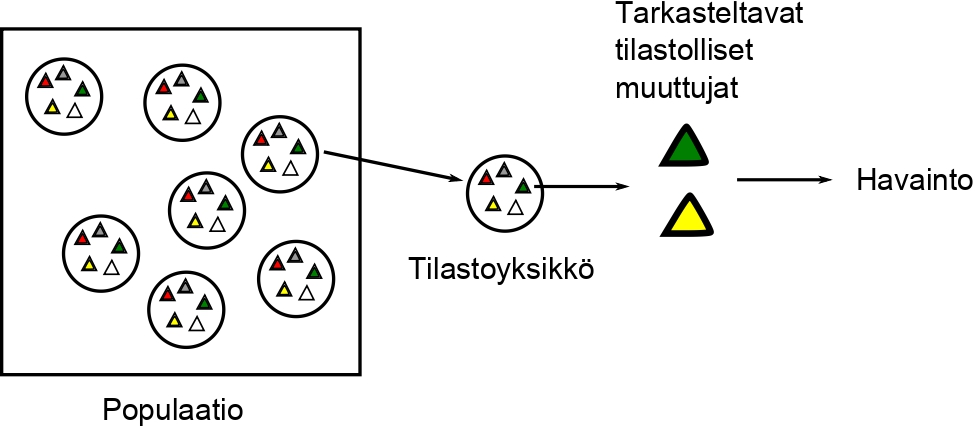
\includegraphics[width=3.69792in,height=\textheight]{populaatiostahavaintoon.jpg}

Tilastollinen tutkimusaineisto, eli havaintoaineisto, koostuu
tilastoyksiköiden muodostamasta populaatioista esimerkiksi otannalla
poimituista alkioista.

Näiltä tilastoyksiköiltä havaitaan tai \textbf{mitataan} tutkimuksessa
tarkasteltavat tilastolliset muuttujat.

\hypertarget{havaintoaineisto}{%
\section{Havaintoaineisto}\label{havaintoaineisto}}

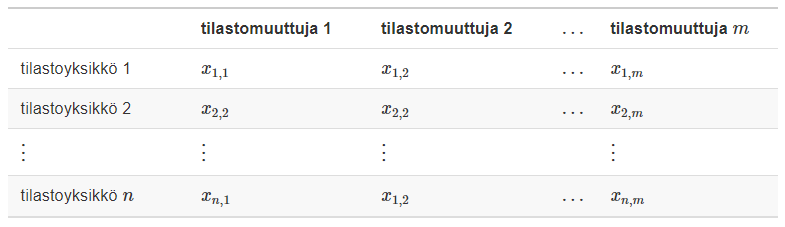
\includegraphics[width=3.86458in,height=\textheight]{havaintoaineisto.png}

Usein havaintoaineisto voidaan koota esimerkiksi yllä olevan kuvan
mukaiseksi taulukoksi.

Tilastoyksiköt ladotaan riveille allekkain ja näihin liitettävät
tilastomuuttujat asetetaan sarakkeisiin. Yo. taulukossa on siis \(n\)
tilastoyksikköä, joista jokaisesta on kerätty \(m\) tilastomuuttujan
arvot.

Tilastollisen muuttujan \(i\) tilastollisesta muuttujasta \(j\) havaittu
arvoa merkitään esimerkiksi \(x_{i,j}\). Varsinaisen tutkimuksen
kannalta mielenkiintoisia muuttujia kutsutaan
\textbf{tutkimusmuuttujiksi} ja muita \textbf{taustamuuttujiksi}.

\hypertarget{keskeiset-termit-kokonaistutkimus-ja-otantatutkimus}{%
\section{Keskeiset termit: kokonaistutkimus ja
otantatutkimus}\label{keskeiset-termit-kokonaistutkimus-ja-otantatutkimus}}

\begin{defblock}{}

\textbf{Kokonaistutkimus}

\begin{itemize}
\tightlist
\item
  Kokonaistutkimus on tutkimus, jossa tutkitaan kaikki tutkimuksen
  kohteena olevan perusjoukon alkiot, ts. kaikki ajateltavissa olevat
  kohteet tutkitaan eli havaintoaineisto koostuu koko populaatiosta.
\end{itemize}

\end{defblock}

\begin{defblock}{}

\textbf{Otantatutkimus}

\begin{itemize}
\item
  Otantatutkimuksessa tutkimus kohdistetaan johonkin populaation, eli
  perusjoukon, osajoukkoon, joka poimitaan sopivaa
  \textbf{otantamenetelmää} käyttäen. Tähän osajoukkoon poimittuja
  alkioita kutsutaan \textbf{otosyksiköiksi} ja koko otosjoukkoa
  \textbf{otokseksi}.
\item
  Tästä osajoukosta tehdään päätelmiä, jotka yleistetään koskemaan koko
  populaatiota/perusjoukkoa.
\end{itemize}

\end{defblock}

\hypertarget{otannan-idea}{%
\section{Otannan idea}\label{otannan-idea}}

Otantatutkimuksen (karkeat) suunnittelu- ja työvaiheet sisältävät mm.
tutkimuksen tavoitteiden asettamisen, näitä vastaavan perusjoukon
asettamisen, otannan suorittamisen sekä lopulta aineiston analysoinnin
ja tulosten raportoimisen.

Tavoitteena on poimia \textbf{edustava otos} mielenkiinnon kohteena
olevasta perusjoukosta, sillä tämä mahdollistaa otoksesta tehtyjen
päätelmien yleistämisen koko perusjoukolle!

\begin{defblock}{}
\textbf{Edustavuus}

Tutkimukseen valittu perusjoukon osajoukko, otos, kuvaa perusjoukon
ominaisuuksia kattavasti.

\end{defblock}

\hypertarget{mittaaminen}{%
\section{Mittaaminen}\label{mittaaminen}}

Kvantitatiivisen tutkimuksen aineistoksi kelpaa kaikki havaintoihin
perustuva informaatio, joka on \textbf{mittauksen} avulla muutettavissa
numeeriseen muotoon. Havaintoyksiköiden tilastollisten muuttujien
numeerisia arvoja kutsutaan \textbf{havaintoarvoiksi} tai
\textbf{havainnoiksi.}

Tilastollisessa tutkimuksessa tilastomuuttujat ovat satunnaisia ja
tavoite on mittaamalla liittää jokin luku satunnaisilmiötä kuvaavaan
ominaisuuteen, eli mitata satunnaismuuttujan havaittua arvoa.

Hyvä mittari on \textbf{(i) validi}, eli mittaus esittää mitattavaa
ominaisuutta oikein ja \textbf{(ii) luotettava}, eli mittaus on
\textbf{harhaton} ja \textbf{toistettavissa}.

Kun käytetään hyviä mittareita, voidaan luotettavuutta vielä erikseen
tarkastella laskemalla aineistosta tunnuslukujua mittauksen
luotettavuudelle, esimerkkinä \textbf{luottamusväli}.

\hypertarget{keskeiset-termit-harhattomuus-ja-toistettavuus}{%
\section{Keskeiset termit: harhattomuus ja
toistettavuus}\label{keskeiset-termit-harhattomuus-ja-toistettavuus}}

\begin{defblock}{}
\textbf{Harhattomuus}

Mittari on harhaton, jos se ei systemaattisesti ali- tai yliarvioi
mitattavan ominaisuuden määrää.

\end{defblock}

\begin{defblock}{}
\textbf{Toistettavuus}

Mittari on toistettava, jos se tuottaa keskimäärin samanlaisia
mittauksia samanlaisista otoksista eli se on johdonmukainen ja
mittausvirheet pieniä.

\end{defblock}

Kun mittaaminen on luotettavaa ja validia, tutkimusaineisto on
\textbf{sisäisesti luotettavaa}.

Aineisto on \textbf{ulkoisesti luotettavaa} silloin, kun tutkittu otos
edustaa perusjoukkoa eli on edustava.

\hypertarget{mitta-asteikot}{%
\section{Mitta-asteikot}\label{mitta-asteikot}}

\textbf{Laatueroasteikko/luokitteluasteikko}: muuttujan mittaustaso on
sellainen, että sen arvot voidaan luokittaa toisistaan eroaviin
luokkiin, mutta luokkien järjestyksellä ei ole merkitystä. Esim:
veriryhmä tai kotikunta. Kvalitatiivinen.

\textbf{Järjestysasteikko} (ordinaaliasteikko): muuttujan arvot voidaan
luokittelun lisäksi asettaa empiirisesti mielekkääseen järjestykseen
mitattavan ominaisuuden perusteella. Esim sotilasarvo, syntymäkuukausi.
Kvalitatiivinen.

\textbf{Välimatka-asteikko} (intervalliasteikko): luokittamisen ja
järjestyksen asettamisen lisäksi havaintoarvojen välimatkalla on
empiirisesti mielekäs tulkinta, ts. arvoista voidaan sanoa kuinka paljon
toinen arvo on toista suurempi. Esim: lämpötila celcius-asteina.
Kvantitatiivinen.

\textbf{Suhdeasteikko:} jos intervalliasteikon ominaisuuksien lisäksi
määriteltynä on yksikäsitteinen mittalukujen absoluuttinen nollapiste,
esimerkiksi kunnan veroäyri tai henkilön pituus: nollapiste on 0.
Kvantitatiivinen.

\hypertarget{kontrolloidut-kokeet-ja-suorat-havainnot}{%
\section{Kontrolloidut kokeet ja suorat
havainnot}\label{kontrolloidut-kokeet-ja-suorat-havainnot}}

\textbf{Kontrolloiduissa kokeissa} tutkimusaineisto kerätään niin, että
tutkimuksen kohteet altistetaan suunnitelmallisesti erilaisiin
koeolosuhteisiin ja selvitetään miten miten kohteet reagoivat
muutoksiin.

\textbf{Suoria havaintoja} käyttäessä tutkimusaineisto kerätään niin,
että koeolosuhteita ei aktiivisesti muuteta, vaan seurataan miten
olosuhteiden muutokset vaikuttavat kohteisiin.

Kummassakin tapauksessa tilastoyksiköihin voi vaikuttaa lisäksi
erilaiset \textbf{selittävät} ja \textbf{sekoittavat tekijät}, joiden
vaikutusten kontrollointi on suoria havaintoja tehdessä vaikeampaa!

\textbf{Puuttuvien selittäjien harhalla} tarkoitetaan tilannetta, jossa
saatuihin tuloksiin vaikuttaa jokin tekijä, jota ei havaita tai jota ei
pystytä mittaamaan ja jonka vaikutusta ei tällöin kyetä kvantifioimaan.

\hypertarget{keskeiset-termit-valikoituminen-ja-satunnaistaminen}{%
\section{Keskeiset termit: valikoituminen ja
satunnaistaminen}\label{keskeiset-termit-valikoituminen-ja-satunnaistaminen}}

\begin{defblock}{}
\textbf{Valikoituminen}

Valikoitumista tapahtuu, jos otokseen poiminta ei ole riippumatonta
tilastoyksikön ominaisuuksista. Tätä kutsutaan valikoitumisharhaksi ja
se estää tulosten luotettavan yleistämisen populaatioon.

\end{defblock}

\begin{defblock}{}
\textbf{Satunnaistaminen}

Tilastoyksiköiden poimimista populaatiosta otokseen riippumatta muiden
yksiköiden poiminnasta tai poimittavien yksiköiden ominaisuuksista.
Satunnaistaminen poistaa valikoitumisharhan takaamalla että mahdolliset
sekoittavat tekijät ovat jakautuneet tasaisesti tutkittavassa joukossa.

\end{defblock}

\hypertarget{otantamenetelmuxe4t}{%
\section{Otantamenetelmät}\label{otantamenetelmuxe4t}}

Otantamenetelmän, joskus myös \textbf{otanta-asetelman}, valinta on
vahvasti sovellusalakohtainen: käytettävät aineistot ja täten
otantamenetelmät määräytyvät pitkälti tehtävän tutkimuksen luonteen
perusteella.

Otanta-asetelmalla tarkoitetaan erityisesti otoksen poimintaan käytettyä
\textbf{satunnaistuksen menetelmää}. Koska tavoitteena on edustava otos,
otannan käytäntöön vaikuttaa se, miten todennäköistä kullakin
perusjoukon alkiolla on tulla poimituksi otokseen.

\begin{defblock}{}
\textbf{Sisältymistodennäköisyys}

Sisältymistodennäköisyys kuvaa sitä (tunnettua) todennäköisyyttä, jolla
perusjoukon alkio tulee poimituksi otokseen. Merkitään \(\pi_k\), jolle
pätee \(0 < \pi_k \leq 1, k = 1,\dots,N\), kun perusjoukon koko on \(N\)
alkiota, ts. jokaisella alkiolla on nollaa suurempi
sisältymistodennäköisyys.

\end{defblock}

Koska sisältymistodennäköisyys voi vaihdella perusjoukon eri
osajoukkojen välillä, tulee tämä huomioida otantamenelmää valitessa!

\hypertarget{yksinkertainen-satunnaisotanta-yso}{%
\section{Yksinkertainen satunnaisotanta
(YSO)}\label{yksinkertainen-satunnaisotanta-yso}}

Yksinkertaista satunnaisotantaa (YSO) pidetään otannan perusmuotona,
jossa jokaisella perusjoukon alkiolla on lähtökohtaisesti yhtä suuri
todennäköisyys tulla valituksi otokseen, ts. sisältymistodennäköisyys ei
riipu tilastoyksikön ominaisuuksista tai otokseen jo valittujen
ominaisuuksista. Korjaa siis valikoitumisharhan!

\textbf{YSO:n toteuttaminen} etenee vaiheittain muodostamalla ensin
lista kaikista perusjoukon alkioista, joista otanta voidaan suorittaa.
Tätä kutsutaan \textbf{otantakehikoksi}. Tämän jälkeen alkiot poimitaan
otokseen yksi kerrallaan satunnaisesti (arpomalla).

\textbf{YSO} voidaan suorittaa joko \textbf{palauttaen} tai
\textbf{palauttamatta,} jotka poikkeavat siinä miten alkioita kohdellaan
sen jälkeen kun ne on poimittu otokseen. Tämä taas vaikuttaa siihen,
miten sisältymistodennäköisyydet muuttuvat otannan edetessä!
Yksityiskohdat löydät luentomateriaalista.

\hypertarget{systemaattinen-otanta}{%
\section{Systemaattinen otanta}\label{systemaattinen-otanta}}

Systemaattisessa, eli tasavälisessä, otannassa perusjoukkoon kuuluvat
alkiot järjestetään jonoon ja siitä poimitaan otokseen joka \(k\).
alkio. Ei oikeastaan satunnaisotantaa, sillä ei hyödynnä arvontaa!

Potentiaalisen ongelman muodostaa havaintoyksikkölistän mahdollisesti
sisältämä säännöllinen jaksollisuus.

Esimerkki: valitaan tehtaan laadunvalvonnassa tuotantolinjalta joka
sadas valmistuva tuote laatuarviointiin.

Mikäli alkiot järjestetään satunnaiseen jonoon, on kyseessä kuitenkin
vain erilainen tapa toteuttaa yksinkertainen satunnaisotanta!

\hypertarget{ositettu-otanta}{%
\section{Ositettu otanta}\label{ositettu-otanta}}

Joskus tutkimuskohteena oleva perusjoukko koostuu jonkin ominaisuuden
suhteen homogeenisista ryhmistä, jotka ovat myös itsessään tutkimuksen
kannalta keskeisiä. Tällöin tulee varmistaa, että tutkittava otos on
edustava kaikkien olennaisten ryhmien osalta.

Esimerkiksi jos tavoitteena on tutkia jonkin maan erilaisten ja usein
hyvin eri kokoisten kieliryhmien taloudellista asemaa ei maan koko
populaatioon kohdistettu YSO olisi järkevää, sillä otoskoon pitäisi
todennäköisesti olla hyvin suuri että jokaisesta kieliryhmästä
saataisiin poimittua edustava otos.

Ositettu otanta ratkaisee ongelman pyrkimällä tunnistamaan tutkimuksen
kannalta keskeiset ryhmät ja suorittamalla YSO näiden ryhmien sisältä ja
yhdistämällä nämä osaotokset yhdeksi otokseksi.

\hypertarget{ryvuxe4sotanta}{%
\section{Ryväsotanta}\label{ryvuxe4sotanta}}

Paikoin tutkimuskohde voidaan jakaa luonnollisiin ryhmiin eli rypäisiin
(eng. \emph{clusters}), jotka indikoivat aineiston luontaista
hierarkkista, eli monitasoista- tai asteista rakennetta.

Esimerkiksi koululuokat muodostavat rypäitä koulujen sisällä ja
koululaiset ovat alkioita omissa rypäissään.

Ryväsotanta usein motivoidaan tietojen keruun aiheuttamien kustannusten
vähentämisellä, sillä rypäiden oletetaan olevan toistensa kanssa
riittävän samankaltaisia, jolloin jokaista rypästä ei tarvitse erikseen
tutkia.

\textbf{Yksivaiheisessa ryväsotannassa} poimitaan joukko rypäitä
kaikkien rypäiden joukosta (satunnaisia kouluja), joiden kaikki alkiot
tutkitaan (valitun koulun kaikki alkiot). \textbf{Kaksivaiheisessa
ryväsotannassa} poimitaan vielä satunnaisesti aliryppäät (valitun koulun
jotkin luokat) ensimmäisen vaiheen rypäiden joukosta, joista otos
poimitaan.

\hypertarget{otannan-haasteita-kootusti}{%
\section{Otannan haasteita kootusti}\label{otannan-haasteita-kootusti}}

Tässä tiivistelmässä ohitettiin keskustelu \textbf{otoskoon}
määrittämisestä. Otoskoko on keskeinen tekijä otoksen edustavuuden
kannalta ja siihen palataan vielä myöhemmissä jaksoissa. Yksi
otantatutkimuksen uhka on ns. \textbf{vastauskato} eli että tutkimuksen
kohteita ei tavoiteta tai he kieltäytyvät vastaamasta, jolloin otoskoko
pienenee.

Otoskehikolla tarkoitetaan sitä perusjoukon osaa, josta otanta
ylipäätään pystytään suorittamaan. \textbf{Otoskehikon yli- tai
alipeitolla} taas tarkoitetaan tilannetta, jossa otantakehikkoon kuuluu
perusjoukkoon kuulumattomia alkioita tai siitä puuttuu osa perusjoukon
alkioista.

\textbf{Poimintaharha}: otos ei edusta populaatiota. Vaarana erityisesti
silloin, kun otokseen tulleet populaation alkiot ovat valikoituneet tai
ovat itse valinneet tiensä otokseen. Aiheutuu myös, kun otoskehikon ali-
tai ylipeitto on liian suuri.



\end{document}
